% Options for packages loaded elsewhere
\PassOptionsToPackage{unicode}{hyperref}
\PassOptionsToPackage{hyphens}{url}
\PassOptionsToPackage{dvipsnames,svgnames,x11names}{xcolor}
%
\documentclass[
  letterpaper,
  DIV=11,
  numbers=noendperiod]{scrreprt}

\usepackage{amsmath,amssymb}
\usepackage{iftex}
\ifPDFTeX
  \usepackage[T1]{fontenc}
  \usepackage[utf8]{inputenc}
  \usepackage{textcomp} % provide euro and other symbols
\else % if luatex or xetex
  \usepackage{unicode-math}
  \defaultfontfeatures{Scale=MatchLowercase}
  \defaultfontfeatures[\rmfamily]{Ligatures=TeX,Scale=1}
\fi
\usepackage{lmodern}
\ifPDFTeX\else  
    % xetex/luatex font selection
\fi
% Use upquote if available, for straight quotes in verbatim environments
\IfFileExists{upquote.sty}{\usepackage{upquote}}{}
\IfFileExists{microtype.sty}{% use microtype if available
  \usepackage[]{microtype}
  \UseMicrotypeSet[protrusion]{basicmath} % disable protrusion for tt fonts
}{}
\makeatletter
\@ifundefined{KOMAClassName}{% if non-KOMA class
  \IfFileExists{parskip.sty}{%
    \usepackage{parskip}
  }{% else
    \setlength{\parindent}{0pt}
    \setlength{\parskip}{6pt plus 2pt minus 1pt}}
}{% if KOMA class
  \KOMAoptions{parskip=half}}
\makeatother
\usepackage{xcolor}
\setlength{\emergencystretch}{3em} % prevent overfull lines
\setcounter{secnumdepth}{5}
% Make \paragraph and \subparagraph free-standing
\makeatletter
\ifx\paragraph\undefined\else
  \let\oldparagraph\paragraph
  \renewcommand{\paragraph}{
    \@ifstar
      \xxxParagraphStar
      \xxxParagraphNoStar
  }
  \newcommand{\xxxParagraphStar}[1]{\oldparagraph*{#1}\mbox{}}
  \newcommand{\xxxParagraphNoStar}[1]{\oldparagraph{#1}\mbox{}}
\fi
\ifx\subparagraph\undefined\else
  \let\oldsubparagraph\subparagraph
  \renewcommand{\subparagraph}{
    \@ifstar
      \xxxSubParagraphStar
      \xxxSubParagraphNoStar
  }
  \newcommand{\xxxSubParagraphStar}[1]{\oldsubparagraph*{#1}\mbox{}}
  \newcommand{\xxxSubParagraphNoStar}[1]{\oldsubparagraph{#1}\mbox{}}
\fi
\makeatother

\usepackage{color}
\usepackage{fancyvrb}
\newcommand{\VerbBar}{|}
\newcommand{\VERB}{\Verb[commandchars=\\\{\}]}
\DefineVerbatimEnvironment{Highlighting}{Verbatim}{commandchars=\\\{\}}
% Add ',fontsize=\small' for more characters per line
\usepackage{framed}
\definecolor{shadecolor}{RGB}{241,243,245}
\newenvironment{Shaded}{\begin{snugshade}}{\end{snugshade}}
\newcommand{\AlertTok}[1]{\textcolor[rgb]{0.68,0.00,0.00}{#1}}
\newcommand{\AnnotationTok}[1]{\textcolor[rgb]{0.37,0.37,0.37}{#1}}
\newcommand{\AttributeTok}[1]{\textcolor[rgb]{0.40,0.45,0.13}{#1}}
\newcommand{\BaseNTok}[1]{\textcolor[rgb]{0.68,0.00,0.00}{#1}}
\newcommand{\BuiltInTok}[1]{\textcolor[rgb]{0.00,0.23,0.31}{#1}}
\newcommand{\CharTok}[1]{\textcolor[rgb]{0.13,0.47,0.30}{#1}}
\newcommand{\CommentTok}[1]{\textcolor[rgb]{0.37,0.37,0.37}{#1}}
\newcommand{\CommentVarTok}[1]{\textcolor[rgb]{0.37,0.37,0.37}{\textit{#1}}}
\newcommand{\ConstantTok}[1]{\textcolor[rgb]{0.56,0.35,0.01}{#1}}
\newcommand{\ControlFlowTok}[1]{\textcolor[rgb]{0.00,0.23,0.31}{\textbf{#1}}}
\newcommand{\DataTypeTok}[1]{\textcolor[rgb]{0.68,0.00,0.00}{#1}}
\newcommand{\DecValTok}[1]{\textcolor[rgb]{0.68,0.00,0.00}{#1}}
\newcommand{\DocumentationTok}[1]{\textcolor[rgb]{0.37,0.37,0.37}{\textit{#1}}}
\newcommand{\ErrorTok}[1]{\textcolor[rgb]{0.68,0.00,0.00}{#1}}
\newcommand{\ExtensionTok}[1]{\textcolor[rgb]{0.00,0.23,0.31}{#1}}
\newcommand{\FloatTok}[1]{\textcolor[rgb]{0.68,0.00,0.00}{#1}}
\newcommand{\FunctionTok}[1]{\textcolor[rgb]{0.28,0.35,0.67}{#1}}
\newcommand{\ImportTok}[1]{\textcolor[rgb]{0.00,0.46,0.62}{#1}}
\newcommand{\InformationTok}[1]{\textcolor[rgb]{0.37,0.37,0.37}{#1}}
\newcommand{\KeywordTok}[1]{\textcolor[rgb]{0.00,0.23,0.31}{\textbf{#1}}}
\newcommand{\NormalTok}[1]{\textcolor[rgb]{0.00,0.23,0.31}{#1}}
\newcommand{\OperatorTok}[1]{\textcolor[rgb]{0.37,0.37,0.37}{#1}}
\newcommand{\OtherTok}[1]{\textcolor[rgb]{0.00,0.23,0.31}{#1}}
\newcommand{\PreprocessorTok}[1]{\textcolor[rgb]{0.68,0.00,0.00}{#1}}
\newcommand{\RegionMarkerTok}[1]{\textcolor[rgb]{0.00,0.23,0.31}{#1}}
\newcommand{\SpecialCharTok}[1]{\textcolor[rgb]{0.37,0.37,0.37}{#1}}
\newcommand{\SpecialStringTok}[1]{\textcolor[rgb]{0.13,0.47,0.30}{#1}}
\newcommand{\StringTok}[1]{\textcolor[rgb]{0.13,0.47,0.30}{#1}}
\newcommand{\VariableTok}[1]{\textcolor[rgb]{0.07,0.07,0.07}{#1}}
\newcommand{\VerbatimStringTok}[1]{\textcolor[rgb]{0.13,0.47,0.30}{#1}}
\newcommand{\WarningTok}[1]{\textcolor[rgb]{0.37,0.37,0.37}{\textit{#1}}}

\providecommand{\tightlist}{%
  \setlength{\itemsep}{0pt}\setlength{\parskip}{0pt}}\usepackage{longtable,booktabs,array}
\usepackage{calc} % for calculating minipage widths
% Correct order of tables after \paragraph or \subparagraph
\usepackage{etoolbox}
\makeatletter
\patchcmd\longtable{\par}{\if@noskipsec\mbox{}\fi\par}{}{}
\makeatother
% Allow footnotes in longtable head/foot
\IfFileExists{footnotehyper.sty}{\usepackage{footnotehyper}}{\usepackage{footnote}}
\makesavenoteenv{longtable}
\usepackage{graphicx}
\makeatletter
\def\maxwidth{\ifdim\Gin@nat@width>\linewidth\linewidth\else\Gin@nat@width\fi}
\def\maxheight{\ifdim\Gin@nat@height>\textheight\textheight\else\Gin@nat@height\fi}
\makeatother
% Scale images if necessary, so that they will not overflow the page
% margins by default, and it is still possible to overwrite the defaults
% using explicit options in \includegraphics[width, height, ...]{}
\setkeys{Gin}{width=\maxwidth,height=\maxheight,keepaspectratio}
% Set default figure placement to htbp
\makeatletter
\def\fps@figure{htbp}
\makeatother

\KOMAoption{captions}{tableheading}
\makeatletter
\@ifpackageloaded{bookmark}{}{\usepackage{bookmark}}
\makeatother
\makeatletter
\@ifpackageloaded{caption}{}{\usepackage{caption}}
\AtBeginDocument{%
\ifdefined\contentsname
  \renewcommand*\contentsname{Table of contents}
\else
  \newcommand\contentsname{Table of contents}
\fi
\ifdefined\listfigurename
  \renewcommand*\listfigurename{List of Figures}
\else
  \newcommand\listfigurename{List of Figures}
\fi
\ifdefined\listtablename
  \renewcommand*\listtablename{List of Tables}
\else
  \newcommand\listtablename{List of Tables}
\fi
\ifdefined\figurename
  \renewcommand*\figurename{Figure}
\else
  \newcommand\figurename{Figure}
\fi
\ifdefined\tablename
  \renewcommand*\tablename{Table}
\else
  \newcommand\tablename{Table}
\fi
}
\@ifpackageloaded{float}{}{\usepackage{float}}
\floatstyle{ruled}
\@ifundefined{c@chapter}{\newfloat{codelisting}{h}{lop}}{\newfloat{codelisting}{h}{lop}[chapter]}
\floatname{codelisting}{Listing}
\newcommand*\listoflistings{\listof{codelisting}{List of Listings}}
\makeatother
\makeatletter
\makeatother
\makeatletter
\@ifpackageloaded{caption}{}{\usepackage{caption}}
\@ifpackageloaded{subcaption}{}{\usepackage{subcaption}}
\makeatother

\ifLuaTeX
  \usepackage{selnolig}  % disable illegal ligatures
\fi
\usepackage{bookmark}

\IfFileExists{xurl.sty}{\usepackage{xurl}}{} % add URL line breaks if available
\urlstyle{same} % disable monospaced font for URLs
\hypersetup{
  pdftitle={Probabilidad II - Práctico},
  pdfauthor={Marco Scavino - Bruno Tancredi},
  colorlinks=true,
  linkcolor={blue},
  filecolor={Maroon},
  citecolor={Blue},
  urlcolor={Blue},
  pdfcreator={LaTeX via pandoc}}


\title{Probabilidad II - Práctico}
\author{Marco Scavino - Bruno Tancredi}
\date{27-04-2025}

\begin{document}
\maketitle

\renewcommand*\contentsname{Table of contents}
{
\hypersetup{linkcolor=}
\setcounter{tocdepth}{2}
\tableofcontents
}

\bookmarksetup{startatroot}

\chapter*{Presentación}\label{presentaciuxf3n}
\addcontentsline{toc}{chapter}{Presentación}

\markboth{Presentación}{Presentación}

Aquí iremos publicando las soluciones de los problemas presentados
durante el curso de Probabilidad II.

\bookmarksetup{startatroot}

\chapter{Problema I}\label{problema-i}

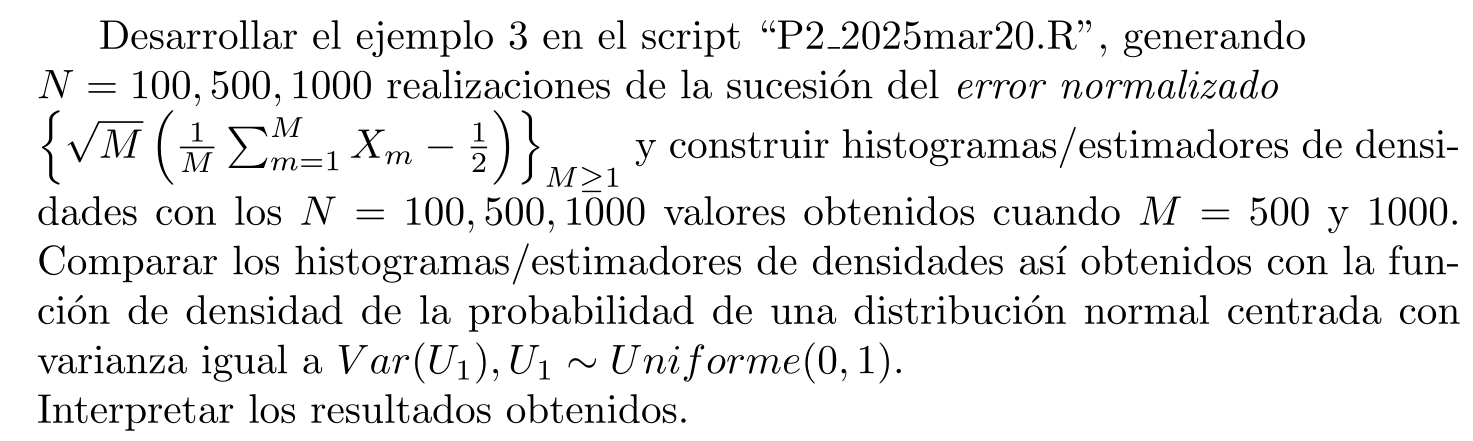
\includegraphics{consignas/problemaI.png}

\section{Enunciado Teorema Central del
Límite}\label{enunciado-teorema-central-del-luxedmite}

Sea \(X_1, X_2, \dots, X_n\) una sucesión de variables aleatorias i.i.d.
con esperanza finita \(\mu\) y varianza finita \(\sigma^2\), y
\(\bar{X}_n = \frac{X_1 + X_2 + \dots + X_n}{n}\).

Entonces, cuando \(n \to \infty\),

\[
\mathbb{P} \left( \frac{\sqrt{n} (\bar{X}_n - \mu)}{\sigma} \leq x \right) \to \Phi(x) \quad \text{para todo } x \in \mathbb{R}
\]

\section{Ejercicio - Solución para N =
1000}\label{ejercicio---soluciuxf3n-para-n-1000}

\begin{Shaded}
\begin{Highlighting}[]
\DocumentationTok{\#\#\# Ejercicio propuesto: desarrollar el ejemplo 3, generando N= 100, 500, 1000 realizaciones de la sucesión del Error normalizado y construir histogramas/estimación de densidades con los 100, 500, 1000 valores obtenidos cuando M = 500 y 1000. Comparar los histogramas/estimación de densidades así obtenidos con la densidad de una distribución normal centrada con varianza igual a Var(U\_1), U\_1 \textasciitilde{} Uniforme(0,1). Interpretar los resultados obtenidos.}

\FunctionTok{rm}\NormalTok{(}\AttributeTok{list=}\FunctionTok{ls}\NormalTok{())}
\FunctionTok{library}\NormalTok{(ggplot2)}
\FunctionTok{library}\NormalTok{(tidyr)}

\CommentTok{\# Establecer semilla global para reproducibilidad}
\FunctionTok{set.seed}\NormalTok{(}\DecValTok{123}\NormalTok{)  }\CommentTok{\# Semilla fija para generar las semillas aleatorias}

\CommentTok{\# Función para generar simulaciones del error normalizado}
\NormalTok{simula\_error\_normalizado }\OtherTok{\textless{}{-}} \ControlFlowTok{function}\NormalTok{(seed, M) \{}
  \FunctionTok{set.seed}\NormalTok{(seed)  }\CommentTok{\# Semilla específica para cada simulación}
\NormalTok{  U }\OtherTok{\textless{}{-}} \FunctionTok{runif}\NormalTok{(M)  }\CommentTok{\# Muestras uniformes}
\NormalTok{  running\_mean }\OtherTok{\textless{}{-}} \FunctionTok{cumsum}\NormalTok{(U) }\SpecialCharTok{/}\NormalTok{ (}\DecValTok{1}\SpecialCharTok{:}\NormalTok{M)  }\CommentTok{\# Media muestral acumulada}
\NormalTok{  norm\_error }\OtherTok{\textless{}{-}} \FunctionTok{sqrt}\NormalTok{(}\DecValTok{1}\SpecialCharTok{:}\NormalTok{M) }\SpecialCharTok{*}\NormalTok{ (running\_mean }\SpecialCharTok{{-}} \FloatTok{0.5}\NormalTok{)  }\CommentTok{\# Error normalizado}
  \FunctionTok{return}\NormalTok{(norm\_error[}\FunctionTok{c}\NormalTok{(}\DecValTok{500}\NormalTok{, }\DecValTok{1000}\NormalTok{, }\DecValTok{2000}\NormalTok{, }\DecValTok{5000}\NormalTok{)])  }\CommentTok{\# Devuelve el error normalizado en M=500, M=1000, M=2000 y M=5000}
\NormalTok{\}}

\CommentTok{\# Parámetros de simulación}
\NormalTok{N }\OtherTok{\textless{}{-}} \DecValTok{1000} \CommentTok{\# 500, 1000 Número de simulaciones}

\CommentTok{\# Generar semillas aleatorias reproducibles}
\NormalTok{semillas }\OtherTok{\textless{}{-}} \FunctionTok{sample}\NormalTok{(}\DecValTok{1}\SpecialCharTok{:}\DecValTok{10}\SpecialCharTok{\^{}}\DecValTok{6}\NormalTok{, N, }\AttributeTok{replace =} \ConstantTok{FALSE}\NormalTok{)}

\CommentTok{\# Generar simulaciones para los valores de M especificados}
\NormalTok{resultados }\OtherTok{\textless{}{-}} \FunctionTok{t}\NormalTok{(}\FunctionTok{sapply}\NormalTok{(semillas, simula\_error\_normalizado, }\AttributeTok{M =} \DecValTok{5000}\NormalTok{))}
\FunctionTok{colnames}\NormalTok{(resultados) }\OtherTok{\textless{}{-}} \FunctionTok{c}\NormalTok{(}\StringTok{"M500"}\NormalTok{, }\StringTok{"M1000"}\NormalTok{, }\StringTok{"M2000"}\NormalTok{, }\StringTok{"M5000"}\NormalTok{)}
\NormalTok{resultados\_df }\OtherTok{\textless{}{-}} \FunctionTok{data.frame}\NormalTok{(resultados)}

\CommentTok{\# identificador ficticio }
\NormalTok{resultados\_df}\SpecialCharTok{$}\NormalTok{id }\OtherTok{\textless{}{-}} \DecValTok{1}\SpecialCharTok{:}\FunctionTok{nrow}\NormalTok{(resultados\_df)}

\CommentTok{\# Transformar a formato largo especificando id.vars}
\NormalTok{resultados\_long }\OtherTok{\textless{}{-}} \FunctionTok{pivot\_longer}\NormalTok{(resultados\_df, }
                        \AttributeTok{cols =} \SpecialCharTok{{-}}\NormalTok{id,}
                        \AttributeTok{names\_to =} \StringTok{\textquotesingle{}M\textquotesingle{}}\NormalTok{,}
                        \AttributeTok{values\_to =} \StringTok{\textquotesingle{}Error\textquotesingle{}}\NormalTok{)}

\CommentTok{\# Convertir la columna \textquotesingle{}M\textquotesingle{} en factor}
\NormalTok{resultados\_long}\SpecialCharTok{$}\NormalTok{M }\OtherTok{\textless{}{-}} \FunctionTok{factor}\NormalTok{(resultados\_long}\SpecialCharTok{$}\NormalTok{M, }
          \AttributeTok{levels =} \FunctionTok{c}\NormalTok{(}\StringTok{"M500"}\NormalTok{, }\StringTok{"M1000"}\NormalTok{, }\StringTok{"M2000"}\NormalTok{, }\StringTok{"M5000"}\NormalTok{),}
          \AttributeTok{labels =} \FunctionTok{c}\NormalTok{(}\StringTok{"M = 500"}\NormalTok{, }\StringTok{"M = 1000"}\NormalTok{, }\StringTok{"M = 2000"}\NormalTok{, }\StringTok{"M = 5000"}\NormalTok{))}

\CommentTok{\# Crear datos para la densidad teórica de la normal con media 0 y varianza 1/12}
\NormalTok{x\_values }\OtherTok{\textless{}{-}} \FunctionTok{seq}\NormalTok{(}\SpecialCharTok{{-}}\FloatTok{1.5}\NormalTok{, }\FloatTok{1.5}\NormalTok{, }\AttributeTok{length.out =} \DecValTok{1000}\NormalTok{)}
\NormalTok{density\_normal }\OtherTok{\textless{}{-}} \FunctionTok{dnorm}\NormalTok{(x\_values, }\AttributeTok{mean =} \DecValTok{0}\NormalTok{, }\AttributeTok{sd =} \FunctionTok{sqrt}\NormalTok{(}\DecValTok{1}\SpecialCharTok{/}\DecValTok{12}\NormalTok{))}

\CommentTok{\# Título dinámico con el valor de N}
\NormalTok{titulo }\OtherTok{\textless{}{-}} \FunctionTok{paste}\NormalTok{(}\StringTok{"Histograma y estimación de densidad del error normalizado}\SpecialCharTok{\textbackslash{}n}\StringTok{"}\NormalTok{, }\StringTok{"con densidad teórica N(0, 1/12) {-} N ="}\NormalTok{, N)}

\CommentTok{\# Gráfico con cuatro paneles}
\NormalTok{plot }\OtherTok{\textless{}{-}} \FunctionTok{ggplot}\NormalTok{(resultados\_long, }\FunctionTok{aes}\NormalTok{(}\AttributeTok{x =}\NormalTok{ Error)) }\SpecialCharTok{+}
  \FunctionTok{geom\_histogram}\NormalTok{(}\FunctionTok{aes}\NormalTok{(}\AttributeTok{y =}\NormalTok{ ..density..), }\AttributeTok{bins =} \DecValTok{30}\NormalTok{, }\AttributeTok{fill =} \StringTok{"blue"}\NormalTok{, }\AttributeTok{alpha =} \FloatTok{0.4}\NormalTok{) }\SpecialCharTok{+}
  \FunctionTok{geom\_density}\NormalTok{(}\AttributeTok{fill =} \StringTok{"blue"}\NormalTok{, }\AttributeTok{alpha =} \FloatTok{0.2}\NormalTok{) }\SpecialCharTok{+}
  \FunctionTok{geom\_line}\NormalTok{(}\AttributeTok{data =} \FunctionTok{data.frame}\NormalTok{(x\_values, density\_normal),}
            \FunctionTok{aes}\NormalTok{(}\AttributeTok{x =}\NormalTok{ x\_values, }\AttributeTok{y =}\NormalTok{ density\_normal),}
            \AttributeTok{color =} \StringTok{"red"}\NormalTok{, }\AttributeTok{linetype =} \StringTok{"dashed"}\NormalTok{, }\AttributeTok{size =} \DecValTok{1}\NormalTok{) }\SpecialCharTok{+}
  \FunctionTok{facet\_wrap}\NormalTok{(}\SpecialCharTok{\textasciitilde{}}\NormalTok{ M, }\AttributeTok{ncol =} \DecValTok{2}\NormalTok{) }\SpecialCharTok{+} \CommentTok{\# Organizar en una cuadrícula de dos columnas}
  \FunctionTok{labs}\NormalTok{(}\AttributeTok{title =}\NormalTok{ titulo,}
       \AttributeTok{x =} \StringTok{"Error normalizado"}\NormalTok{,}
       \AttributeTok{y =} \StringTok{"Densidad"}\NormalTok{) }\SpecialCharTok{+}
  \FunctionTok{theme\_minimal}\NormalTok{() }\SpecialCharTok{+}
  \FunctionTok{theme}\NormalTok{(}\AttributeTok{strip.text =} \FunctionTok{element\_text}\NormalTok{(}\AttributeTok{face =} \StringTok{"bold"}\NormalTok{))}
\NormalTok{plot}
\end{Highlighting}
\end{Shaded}

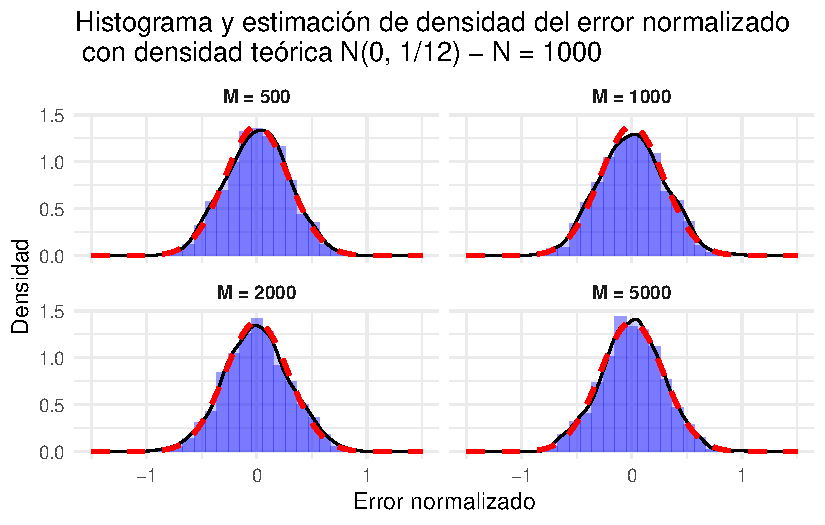
\includegraphics{problema_I_files/figure-pdf/unnamed-chunk-1-1.pdf}

\section{Recomendación}\label{recomendaciuxf3n}

\url{https://www.youtube.com/watch?v=zeJD6dqJ5lo}

\bookmarksetup{startatroot}

\chapter{Problema II}\label{problema-ii}

Queremos estimar la función generatriz de momentos (transformada de
Laplace)

\[
\phi_{X}(u):=E[e^{uX}], u \in \mathbb{R}
\]

de una variable aleatoria \(X\sim N(0,\sigma^{2})\) utilizando una
muestra de tamaño M de copias i.i.d. de X. El parámetro \(\sigma^{2}\)
es desconocido.

\begin{enumerate}
\def\labelenumi{\arabic{enumi}.}
\item
  Demostrar que para \(X\sim N(0,\sigma^{2})\) se cumple: \[
    \mathbb{E}[e^{uX}]=e^{\sigma^{2}u^{2}/2}
  \]
\item
  Comparar la precisión de los siguientes dos estimadores de
  \(\phi_{X}(u)\):\\
  \textbf{\emph{Estimador directo:}} \[
    \phi_{1,M}(u):=\frac{1}{M}\sum_{m=1}^{M}e^{uX_{m}}.
  \] \textbf{\emph{Estimador en dos etapas:}}

  \begin{enumerate}
  \def\labelenumii{\alph{enumii})}
  \tightlist
  \item
    Estimar \(\sigma^{2}\) mediante: \[
       \sigma_{M}^{2}=\frac{1}{M-1}\sum_{m=1}^{M}(X_{m}-\bar{X})^{2}
    \]
  \item
    Construir el estimador `plug-in` de \(\phi_{X}(u)\) \[
      \phi_{2,M}(u):=e^{\frac{u^{2}}{2}\sigma_{M}^{2}}
    \]
  \end{enumerate}
\end{enumerate}

Construir intervalos de confianza asintóticos para ambos estimadores de
\(\phi_{X}(u)\). Interpretar los resultados obtenidos.

\section{Parte 1}\label{parte-1}

\$\$

\begin{aligned}

\mathbb{E} \left[ e^{uX} \right] 

&= \int_{-\infty}^{+\infty} e^{ux}\frac{1}{\sqrt{2\pi\sigma^2}}e^{\frac{-x^2}{2\sigma^2}}dx \\ 

&= \int_{-\infty}^{+\infty} \frac{1}{\sqrt{2\pi\sigma^2}}e^{\frac{-1}{2\sigma^2}[x^2 - 2\sigma^2ux]}dx \\

&= \int_{-\infty}^{+\infty} \frac{1}{\sqrt{2\pi\sigma^2}}e^{\frac{-1}{2\sigma^2}[x^2 - 2\sigma^2ux + (\sigma^2u)^2 - (\sigma^2u)^2]} dx \\

&=  \int_{-\infty}^{+\infty} \frac{1}{\sqrt{2\pi\sigma^2}}e^{\frac{-1}{2\sigma^2}[(x -u\sigma^2)^2 -(u\sigma^2)^2]}dx \\

&= e^\frac{(u\sigma^2)^2}{2\sigma^2}\int_{-\infty}^{+\infty}\frac{1}{\sqrt{2\pi\sigma^2}}e^\frac{-(x-u\sigma^2)^2}{2\sigma^2}\\

&\text{Lo que nos queda dentro de la integral es la densidad de una } \mathcal{N}(u\sigma^2, \sigma^2) \text{ por lo que integra 1} \\

&= e^\frac{u^2\sigma^2}{2}

\end{aligned}

\$\$

\section{Parte 2}\label{parte-2}




\end{document}
